% Paper (Springer LNCS). Compilar desde esta carpeta:  latexmk -pdf paper.tex
% Cifras: ../numeros.tex; filas de tablas: ../tablas.tex (generados por ../analisis.py).
\documentclass[runningheads]{llncs}
\usepackage[T1]{fontenc}
\usepackage[utf8]{inputenc}
\usepackage[spanish,es-tabla,es-nodecimaldot]{babel}
\usepackage{amsmath,amssymb}
\usepackage{graphicx}
\usepackage{booktabs}
\usepackage{xcolor}
\usepackage{tikz}
\usetikzlibrary{arrows.meta,positioning}
\usepackage[hidelinks]{hyperref}
\definecolor{azulm}{HTML}{2E6DB4}\definecolor{naranjam}{HTML}{D9731A}
\definecolor{verdem}{HTML}{2F9467}\definecolor{grism}{HTML}{5A6772}
\graphicspath{{../figuras/}}
% Generado por analisis.py: NO editar a mano.
\newcommand{\nDatasets}{12}
\newcommand{\nParticiones}{5}
\newcommand{\cambioRL}{$-$14{,}6\,\%}
\newcommand{\dsRL}{11/12}
\newcommand{\pRL}{$0{,}027$}
\newcommand{\pSinHolmRL}{$0{,}003$}
\newcommand{\vsEstRL}{$-$13{,}1\,\%}
\newcommand{\pVsEstRL}{$0{,}027$}
\newcommand{\peorRL}{$+$1{,}2\,\%}
\newcommand{\peorDsRL}{kin8nm}
\newcommand{\cambioKNN}{$-$21{,}2\,\%}
\newcommand{\dsKNN}{9/12}
\newcommand{\pKNN}{$0{,}161$}
\newcommand{\pSinHolmKNN}{$0{,}027$}
\newcommand{\vsEstKNN}{$-$10{,}0\,\%}
\newcommand{\pVsEstKNN}{$0{,}386$}
\newcommand{\peorKNN}{$+$28{,}5\,\%}
\newcommand{\peorDsKNN}{kin8nm}
\newcommand{\cambioArbol}{$-$0{,}6\,\%}
\newcommand{\dsArbol}{5/12}
\newcommand{\pArbol}{$1{,}000$}
\newcommand{\pSinHolmArbol}{$0{,}910$}
\newcommand{\vsEstArbol}{$-$0{,}7\,\%}
\newcommand{\pVsEstArbol}{$1{,}000$}
\newcommand{\peorArbol}{$+$6{,}7\,\%}
\newcommand{\peorDsArbol}{kin8nm}
\newcommand{\cambioRF}{$+$0{,}3\,\%}
\newcommand{\dsRF}{5/12}
\newcommand{\pRF}{$1{,}000$}
\newcommand{\pSinHolmRF}{$0{,}733$}
\newcommand{\vsEstRF}{$+$0{,}3\,\%}
\newcommand{\pVsEstRF}{$1{,}000$}
\newcommand{\peorRF}{$+$12{,}4\,\%}
\newcommand{\peorDsRF}{kin8nm}
\newcommand{\cambioMedio}{$-$9{,}5\,\%}
\newcommand{\sinKinRL}{$-$15{,}9\,\%}
\newcommand{\pSinKinRL}{$0{,}004$}
\newcommand{\sinKinKNN}{$-$24{,}6\,\%}
\newcommand{\pSinKinKNN}{$0{,}021$}
\newcommand{\sinKinArbol}{$-$1{,}3\,\%}
\newcommand{\pSinKinArbol}{$1{,}000$}
\newcommand{\sinKinRF}{$-$0{,}8\,\%}
\newcommand{\pSinKinRF}{$1{,}000$}
\newcommand{\sinKinMedio}{$-$11{,}2\,\%}
\newcommand{\maxRL}{$-$59{,}6\,\%}
\newcommand{\maxDsRL}{cpu\_small}
\newcommand{\maxKNN}{$-$58{,}7\,\%}
\newcommand{\maxDsKNN}{california}
\newcommand{\maxArbol}{$-$9{,}8\,\%}
\newcommand{\maxDsArbol}{space\_ga}
\newcommand{\maxRF}{$-$11{,}7\,\%}
\newcommand{\maxDsRF}{space\_ga}
\newcommand{\maxMaeOrig}{6{,}25}
\newcommand{\maxMaeP}{2{,}52}
\newcommand{\dimMedia}{83\,\%}
\newcommand{\origMedia}{4{,}9}
\newcommand{\compMedia}{2{,}2}
\newcommand{\fracComp}{93\,\%}
\newcommand{\fracElim}{43\,\%}
\newcommand{\siempreMenor}{sí}
\newcommand{\segMediana}{292}
\newcommand{\segMax}{438}
\newcommand{\cribCasos}{14}
\newcommand{\cribP}{0{,}900}
\newcommand{\cribPSeg}{199}
\newcommand{\cribPKNN}{0{,}758}
\newcommand{\cribKnn}{0{,}909}
\newcommand{\cribKnnSeg}{113}
\newcommand{\cribKnnKNN}{0{,}740}
\newcommand{\cribMinimax}{0{,}939}
\newcommand{\cribMinimaxSeg}{234}
\newcommand{\cribMinimaxKNN}{0{,}824}
\newcommand{\cribFamilia}{0{,}893}
\newcommand{\cribFamiliaSeg}{121}
\newcommand{\cribFamiliaKNN}{0{,}740}
\newcommand{\cribParada}{0{,}928}
\newcommand{\cribParadaSeg}{69}
\newcommand{\cribParadaKNN}{0{,}794}
\newcommand{\cribParadaTreinta}{0{,}923}
\newcommand{\cribParadaTreintaSeg}{84}
\newcommand{\cribParadaTreintaKNN}{0{,}794}
\newcommand{\cribSeleccion}{0{,}923}
\newcommand{\cribSeleccionSeg}{95}
\newcommand{\cribSeleccionKNN}{0{,}795}
\newcommand{\ablCasos}{24}
\newcommand{\ablKnn}{$+$1{,}4\,\%}
\newcommand{\ablKnnRL}{$+$12{,}2\,\%}
\newcommand{\ablKnnKNN}{$-$3{,}2\,\%}
\newcommand{\ablKnnArbol}{$-$2{,}1\,\%}
\newcommand{\ablKnnRF}{$-$0{,}5\,\%}
\newcommand{\ablKnnDim}{0{,}83}
\newcommand{\ablSinSint}{$-$0{,}2\,\%}
\newcommand{\ablSinSintRL}{$+$0{,}2\,\%}
\newcommand{\ablSinSintKNN}{$-$1{,}4\,\%}
\newcommand{\ablSinSintArbol}{$+$0{,}5\,\%}
\newcommand{\ablSinSintRF}{$+$0{,}1\,\%}
\newcommand{\ablSinSintDim}{0{,}77}
\newcommand{\ablSinForma}{$+$4{,}1\,\%}
\newcommand{\ablSinFormaRL}{$+$14{,}1\,\%}
\newcommand{\ablSinFormaKNN}{$+$2{,}2\,\%}
\newcommand{\ablSinFormaArbol}{$+$0{,}0\,\%}
\newcommand{\ablSinFormaRF}{$+$0{,}6\,\%}
\newcommand{\ablSinFormaDim}{0{,}75}
\newcommand{\ablSinLimite}{$-$0{,}6\,\%}
\newcommand{\ablSinLimiteRL}{$+$0{,}4\,\%}
\newcommand{\ablSinLimiteKNN}{$-$1{,}3\,\%}
\newcommand{\ablSinLimiteArbol}{$-$1{,}1\,\%}
\newcommand{\ablSinLimiteRF}{$-$0{,}6\,\%}
\newcommand{\ablSinLimiteDim}{1{,}32}
\newcommand{\ablAleat}{$+$3{,}5\,\%}
\newcommand{\ablAleatRL}{$+$4{,}5\,\%}
\newcommand{\ablAleatKNN}{$+$5{,}5\,\%}
\newcommand{\ablAleatArbol}{$+$1{,}9\,\%}
\newcommand{\ablAleatRF}{$+$2{,}1\,\%}
\newcommand{\ablAleatDim}{0{,}82}
\newcommand{\ablAG}{$+$0{,}0\,\%}
\newcommand{\ablAGRL}{$+$0{,}3\,\%}
\newcommand{\ablAGKNN}{$+$0{,}7\,\%}
\newcommand{\ablAGArbol}{$-$0{,}2\,\%}
\newcommand{\ablAGRF}{$-$0{,}7\,\%}
\newcommand{\ablAGDim}{0{,}85}
\newcommand{\rangoP}{3{,}6}
\newcommand{\posP}{1}
\newcommand{\rangoPG}{4{,}0}
\newcommand{\compPGRL}{$-$15{,}7\,\%}
\newcommand{\compPGKNN}{$-$18{,}0\,\%}
\newcommand{\compPGArbol}{$+$0{,}7\,\%}
\newcommand{\compPGRF}{$+$0{,}8\,\%}
\newcommand{\rangoEstPCA}{4{,}1}
\newcommand{\compEstPCARL}{$-$1{,}8\,\%}
\newcommand{\compEstPCAKNN}{$-$12{,}4\,\%}
\newcommand{\compEstPCAArbol}{$-$0{,}6\,\%}
\newcommand{\compEstPCARF}{$-$1{,}9\,\%}
\newcommand{\rangoMLKR}{5{,}2}
\newcommand{\compMLKRRL}{$-$1{,}8\,\%}
\newcommand{\compMLKRKNN}{$-$22{,}5\,\%}
\newcommand{\compMLKRArbol}{$+$2{,}0\,\%}
\newcommand{\compMLKRRF}{$+$2{,}6\,\%}
\newcommand{\rangoPCA}{7{,}2}
\newcommand{\compPCARL}{$+$0{,}6\,\%}
\newcommand{\compPCAKNN}{$-$10{,}4\,\%}
\newcommand{\compPCAArbol}{$+$19{,}3\,\%}
\newcommand{\compPCARF}{$+$17{,}9\,\%}
\newcommand{\rangoYJMV}{4{,}3}
\newcommand{\compYJMVRL}{$+$2{,}4\,\%}
\newcommand{\compYJMVKNN}{$-$14{,}5\,\%}
\newcommand{\compYJMVArbol}{$+$1{,}5\,\%}
\newcommand{\compYJMVRF}{$+$1{,}7\,\%}
% Generado por analisis.py.
\newcommand{\filasPrincipal}{%
R. lineal & 0{,}98 & \textbf{0{,}85} & 11/12 & $0{,}027$ & $-$13{,}1\,\% & $0{,}027$\\
KNN & 0{,}88 & \textbf{0{,}79} & 9/12 & $0{,}161$ & $-$10{,}0\,\% & $0{,}386$\\
Árbol & 1{,}00 & \textbf{0{,}99} & 5/12 & $1{,}000$ & $-$0{,}7\,\% & $1{,}000$\\
RF & 1{,}00 & \textbf{1{,}00} & 5/12 & $1{,}000$ & $+$0{,}3\,\% & $1{,}000$\\
}
\newcommand{\filasDimension}{%
diabetes & 10 & 6{,}2 & 2{,}8 & 9{,}0\\
california & 8 & 5{,}0 & 2{,}0 & 7{,}0\\
concrete & 8 & 5{,}8 & 1{,}0 & 6{,}8\\
stock & 9 & 6{,}4 & 1{,}6 & 8{,}0\\
space\_ga & 6 & 2{,}8 & 2{,}2 & 5{,}0\\
sulfur & 6 & 3{,}0 & 2{,}0 & 5{,}0\\
kin8nm & 8 & 4{,}6 & 2{,}4 & 7{,}0\\
bank8FM & 8 & 3{,}6 & 3{,}4 & 7{,}0\\
puma8NH & 8 & 2{,}2 & 0{,}6 & 2{,}8\\
house\_8L & 8 & 5{,}4 & 1{,}6 & 7{,}0\\
cpu\_small & 12 & 7{,}2 & 3{,}8 & 11{,}0\\
wine\_quality & 11 & 7{,}0 & 3{,}0 & 10{,}0\\
}
\newcommand{\filasCribado}{%
\textbf{$P$: KNN+RL+árbol} & 0{,}91 & 0{,}76 & 0{,}96 & 0{,}99 & 0{,}900 & 0{,}993 & 199\\
fitness solo KNN & 0{,}96 & 0{,}74 & 0{,}97 & 0{,}99 & 0{,}909 & 0{,}992 & 113\\
fitness minimax & 0{,}94 & 0{,}82 & 0{,}99 & 1{,}01 & 0{,}939 & 1{,}012 & 234\\
un fitness por familia & 0{,}90 & 0{,}74 & 0{,}96 & 1{,}00 & 0{,}893 & 1{,}002 & 121\\
+ parada (pac.\ 15) & 0{,}91 & 0{,}79 & 1{,}00 & 1{,}03 & 0{,}928 & 1{,}028 & 69\\
+ parada (pac.\ 30) & 0{,}91 & 0{,}79 & 0{,}99 & 1{,}02 & 0{,}923 & 1{,}022 & 84\\
+ elegir $\theta$ con apartado & 0{,}91 & 0{,}80 & 0{,}99 & 1{,}02 & 0{,}923 & 1{,}021 & 95\\
}
\newcommand{\filasAblacion}{%
fitness solo KNN & $+$12{,}2\,\%$^*$ & $-$3{,}2\,\% & $-$2{,}1\,\% & $-$0{,}5\,\% & $+$1{,}4\,\% & 0{,}83\\
sin síntesis & $+$0{,}2\,\% & $-$1{,}4\,\% & $+$0{,}5\,\% & $+$0{,}1\,\% & $-$0{,}2\,\% & 0{,}77\\
sin forma ($\lambda$ = 1) & $+$14{,}1\,\%$^*$ & $+$2{,}2\,\% & $+$0{,}0\,\% & $+$0{,}6\,\% & $+$4{,}1\,\% & 0{,}75\\
sin límite n$-$1 & $+$0{,}4\,\% & $-$1{,}3\,\% & $-$1{,}1\,\% & $-$0{,}6\,\% & $-$0{,}6\,\% & 1{,}32\\
búsqueda aleatoria & $+$4{,}5\,\%$^*$ & $+$5{,}5\,\% & $+$1{,}9\,\% & $+$2{,}1\,\% & $+$3{,}5\,\% & 0{,}82\\
algoritmo genético & $+$0{,}3\,\% & $+$0{,}7\,\% & $-$0{,}2\,\% & $-$0{,}7\,\% & $+$0{,}0\,\% & 0{,}85\\
}
\newcommand{\filasComparativa}{%
estándar & 0{,}98$^*$ & 0{,}88 & 1{,}00 & 1{,}00 & 4{,}6 & 1{,}00\\
YJ máx.\ verosimilitud & 1{,}02$^*$ & 0{,}85 & 1{,}01 & 1{,}02 & 4{,}3 & 1{,}00\\
cuantiles & 1{,}08$^*$ & 0{,}88 & 1{,}00 & 1{,}00 & 5{,}5 & 1{,}00\\
solo PCA (95\,\%) & 1{,}01$^*$ & 0{,}90 & 1{,}19$^*$ & 1{,}18 & 7{,}2 & 0{,}79\\
solo PCA (\% por VC) & 0{,}99$^*$ & 0{,}88 & 1{,}19$^*$ & 1{,}15 & 6{,}6 & 0{,}91\\
estándar + su PCA & 0{,}98$^*$ & 0{,}88 & 0{,}99 & \textbf{0{,}98} & 4{,}1 & 2{,}00\\
MLKR & 0{,}98$^*$ & \textbf{0{,}78} & 1{,}02 & 1{,}03 & 5{,}2 & 1{,}00\\
prog.\ genética & \textbf{0{,}84} & 0{,}82 & 1{,}01 & 1{,}01 & 4{,}0 & 2{,}00\\
\textbf{$P$} & 0{,}85 & 0{,}79 & \textbf{0{,}99} & 1{,}00 & 3{,}6 & 0{,}83\\
}

\setlength{\textfloatsep}{10pt plus 2pt}

\begin{document}
\title{Aumentar, ponderar y reducir: aprendizaje evolutivo de una representación de atributos más pequeña para
regresión}
\titlerunning{Aumentar, ponderar y reducir}
\author{Andrea López Salazar}
\authorrunning{A. López Salazar}
\institute{Universidad Carlos III de Madrid, Máster en Ciencia y Tecnología}
\maketitle

\begin{abstract}
Proponemos un método que aprende, solo con el conjunto de entrenamiento, una representación de atributos con
\emph{menos} dimensiones que la original y que reduce el error de modelos de regresión de familias distintas. Se
aumenta el espacio con las componentes principales de los atributos (con su forma corregida por Yeo-Johnson), se
pondera cada uno de los $2n$ candidatos y se conservan los de peso mayor que un umbral, como mucho $n-1$. CMA-ES
optimiza exponentes, pesos y umbral sobre la media del error normalizado de KNN, regresión lineal y un árbol. En
\nDatasets{} datasets y \nParticiones{} particiones no usadas en el diseño, la representación usa el \dimMedia{} de
los atributos y el error baja un \cambioRL{} en regresión lineal ($p=$\pRL) y un \cambioKNN{} en KNN, con reducciones de
hasta \maxRL{}; en los árboles queda igual. Tiene el mejor rango medio frente a ocho transformaciones conocidas, y
cada decisión de diseño se contrasta con una alternativa.
\keywords{CMA-ES \and reducción de dimensionalidad \and síntesis de atributos \and Yeo-Johnson \and regresión}
\end{abstract}

\section{Introducción}
Dado $(X_t,y_t)$, buscamos un programa $P$ que, con computación evolutiva, aprenda $X\mapsto X'$ con síntesis de
atributos y $\dim X'<\dim X$, tal que un modelo \emph{arbitrario} $M$ entrenado con $X'_t$ tenga menor error absoluto
medio en validación ($e'<e$). KNN depende de la geometría, la regresión lineal (RL) de la forma de cada atributo y un
árbol, invariante a cambios monótonos por atributo, solo de las direcciones por las que corta. Contribuciones: (i) una
representación ``aumentar, ponderar y reducir'' en la que la restricción de dimensión se cumple por construcción y el
criterio de eliminación lo aprende CMA-ES~\cite{hansen2001}; (ii) un fitness con tres familias de modelos; (iii) una
evaluación en dos fases, con estadística por dataset, ablaciones de cada pieza y comparación con ocho alternativas.

\section{Trabajos relacionados}
Ponderar atributos para KNN es una idea clásica~\cite{wettschereck1997}, y los algoritmos genéticos se han usado para
aprender pesos y seleccionar atributos~\cite{raymer2000}. El aprendizaje de métricas~\cite{weinberger2009} usa una
matriz completa, sin corregir la forma de cada atributo. Las transformaciones de potencia~\cite{yeo2000} se ajustan
normalmente por máxima verosimilitud; aquí sus exponentes se eligen para predecir. Añadir componentes principales para
dar cortes oblicuos a los árboles es la idea de Rotation Forest~\cite{rodriguez2006}.

\section{Método}
Para cada atributo, $\tilde x_j=(\psi(x_j;\lambda_j)-\mu_j)/\sigma_j$, con $\psi$ la transformación de Yeo-Johnson,
$\lambda_j\in[-2,2]$ y $\mu_j,\sigma_j$ del entrenamiento. Con $V$ las componentes principales de $\tilde x$, los $2n$
candidatos son $c=[\tilde x\mid \mathrm{std}(V^\top\tilde x)]$ y
\begin{equation}
S=\mathrm{top}_{n-1}\{k: v_k\ge\tau\},\qquad X'=[\,v_k c_k\,]_{k\in S},\qquad v_k,\tau\in[0,3],
\end{equation}
donde $\mathrm{top}_{n-1}$ conserva los $n-1$ de mayor peso si hay más (y el de mayor peso si no queda ninguno): $\dim
X'\le n-1$ para cualquier $\theta=(\lambda,v,\tau)$, con $3n+1$ genes (Fig.~\ref{fig:esquema}).

\begin{figure}[t]\centering\def\esquemaescala{0.75}
% Esquema del método P (aumentar -> ponderar -> reducir), compartido por memoria, paper y póster.
% Requiere tikz con arrows.meta y positioning; colores azulm, naranjam, verdem, grism.
\providecommand{\esquemaescala}{1}
\begin{tikzpicture}[scale=\esquemaescala, every node/.style={transform shape},
  node distance=3.5mm and 4mm,
  caja/.style={draw=azulm, rounded corners=2pt, fill=azulm!8, align=center, inner sep=2.5pt,
               minimum height=9mm, font=\footnotesize},
  sint/.style={caja, draw=verdem, fill=verdem!10},
  red/.style={caja, draw=naranjam, fill=naranjam!8},
  fl/.style={-{Stealth[length=2mm]}, thick, azulm!80!black},
  fv/.style={fl, verdem!80!black},
  fn/.style={fl, naranjam!80!black}]
\node (x) {$X$};
\node[caja, right=of x] (yj) {1. Forma\\$\psi(x_j;\lambda_j)$, estandarizar};
\node[sint, right=of yj] (aum) {2. Aumentar ($2n$)\\$c=[\,\tilde x_1..\tilde x_n \mid p_1..p_n\,]$};
\node[caja, below=7mm of aum] (pes) {3. Pesos dobles\\$v_k\,c_k$,\; $k=1..2n$};
\node[red, left=of pes] (red) {4. Reducir\\$v_k\ge\tau$, como mucho $n-1$};
\node[draw=grism, thick, rounded corners=2pt, fill=white, font=\footnotesize, minimum height=7mm,
      left=of red] (xp) {$X'$,\; $\dim X'<n$};
\draw[fl] (x)--(yj); \draw[fv] (yj)--(aum); \draw[fl] (aum)--(pes); \draw[fn] (pes)--(red); \draw[fn] (red)--(xp);
\node[font=\scriptsize\itshape, text=grism, align=left, anchor=west] at ([xshift=8mm]aum.east)
     {$p$: componentes\\principales de $\tilde x$};
\coordinate (r) at ([xshift=5mm]aum.east);
\node[caja, draw=naranjam, fill=naranjam!10, above=6mm of yj.north east, anchor=south, align=center] (cma)
     {CMA-ES busca $\theta=(\lambda,v,\tau)$ ($3n+1$ genes) minimizando la media del MAE normalizado\\
      de validación cruzada de \textbf{KNN, regresión lineal y árbol} en el entrenamiento};
\draw[fn] (cma.south -| yj) -- (yj.north);
\draw[fn] (cma.south -| r) -- (r |- pes.east) -- (pes.east);
\end{tikzpicture}

\caption{El programa $P$: aumentar a $2n$ candidatos, ponderarlos y conservar como mucho $n-1$.}
\label{fig:esquema}
\end{figure}

\textbf{Fitness.} Media, sobre KNN ($k=5$), RL y un árbol de decisión, del MAE de validación cruzada (5 pliegues
fijos) dividido por el MAE de predecir la mediana, en una submuestra de hasta 2000 filas. El árbol representa a la
familia de Random Forest (RF), cuyo coste por evaluación sería diez veces mayor.
\textbf{Búsqueda.} CMA-ES en $[0,1]^{3n+1}$ reescalado a los límites: selección por rango (invariante a
transformaciones monótonas del fitness), recombinación intermedia ponderada (promedia el ruido de la validación
cruzada) y adaptación de $\sigma$ y de la covarianza (aprende genes acoplados), con $\sigma_0=0{,}2$, población por
defecto y 1000 evaluaciones, desde estandarizar sin componentes.

\section{Diseño experimental}
Doce datasets de regresión (diabetes, california y diez de OpenML; 6--12 atributos, $\le$10\,000 filas). Las
decisiones se tomaron en un cribado con semillas de exploración (0--1, siete datasets); el método se mide en cinco
particiones 70/30 nuevas (semillas 40--44). Modelos fijos: RL, KNN, árbol y RF (100 árboles). Como las particiones de
un dataset comparten filas, la unidad es el dataset: $e'/e$ con media geométrica, Wilcoxon con Holm y Friedman con
Nemenyi~\cite{demsar2006}. No se excluye ningún dataset.

\section{Resultados}
\begin{table}[tb]\centering\setlength{\tabcolsep}{5pt}
\caption{$e'/e$ en las particiones de confirmación (media geométrica de 12 datasets). $p$: Wilcoxon por dataset con
Holm, frente a $X$ original y frente a $X$ estandarizado.}
\label{tab:principal}
\begin{tabular}{@{}lcccccc@{}}\toprule
Modelo & estándar & $P$ & Datasets & $p$ & vs.\ estándar & $p$\\\midrule
\filasPrincipal\bottomrule
\end{tabular}
\end{table}
\textbf{Resultado principal.} Con $\dim X'<n$ (Tabla~\ref{tab:principal}, Fig.~\ref{fig:principal}), RL mejora
\cambioRL{} (\dsRL{} datasets) y KNN \cambioKNN{} (\dsKNN), con máximos de \maxRL{} (\maxDsRL) y \maxKNN{}
(\maxDsKNN). Los árboles quedan igual (árbol \cambioArbol, RF \cambioRF). KNN pierde la significación tras Holm por
\peorDsKNN{} (\peorKNN), donde todos los atributos importan por igual; sin él, como análisis de sensibilidad, KNN
mejora \sinKinKNN{} ($p=$\pSinKinKNN). $X'$ conserva de media \origMedia{} originales y \compMedia{} componentes
(\dimMedia{} de $n$), con componentes en el \fracComp{} de las particiones.

\begin{figure}[tb]\centering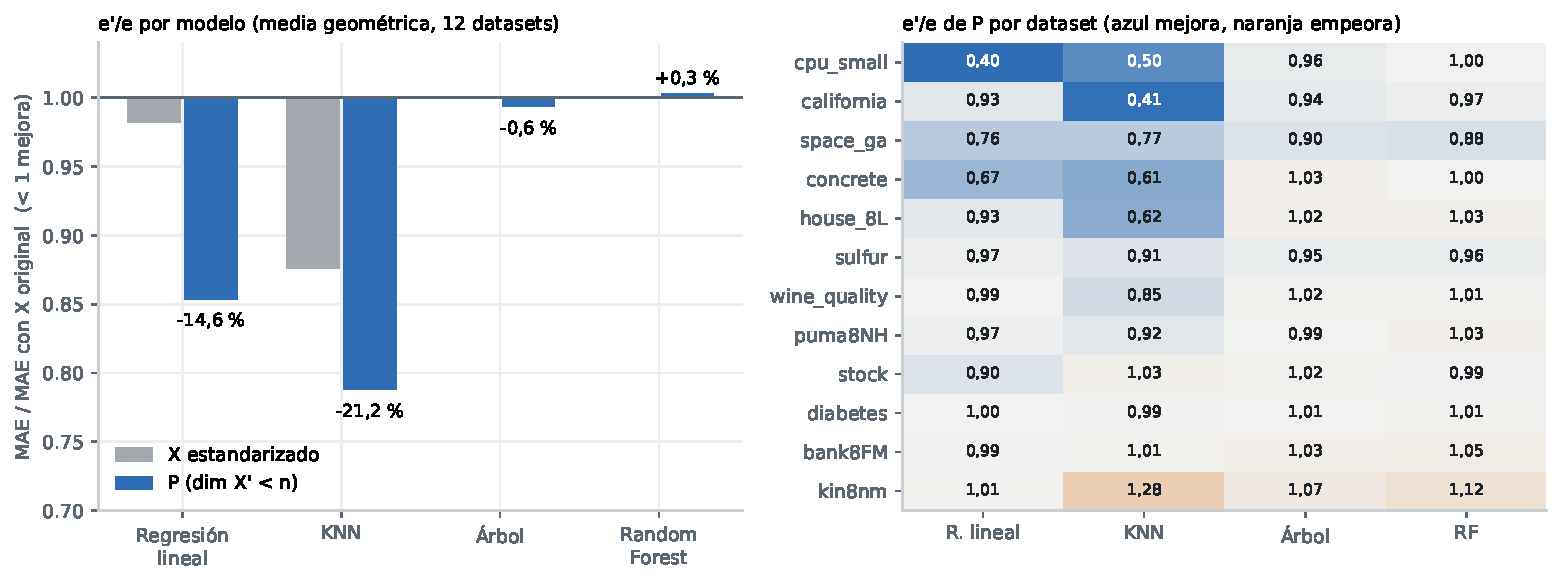
\includegraphics[width=\textwidth]{principal}
\caption{Izquierda: $e'/e$ por modelo. Derecha: $e'/e$ de $P$ por dataset (azul: mejora; naranja: empeora).}
\label{fig:principal}
\end{figure}

\begin{table}[tb]\centering\setlength{\tabcolsep}{4pt}
\caption{Cribado de diseño (\cribCasos{} particiones de exploración): $e'/e$ por modelo, media, peor modelo y
segundos por búsqueda.}
\label{tab:cribado}\scriptsize
\begin{tabular}{@{}lccccccc@{}}\toprule
Variante & RL & KNN & Árbol & RF & media & peor & s\\\midrule
\filasCribado\bottomrule
\end{tabular}
\end{table}
\textbf{Diseño.} En el cribado (Tabla~\ref{tab:cribado}), el fitness de tres familias mejora la media (\cribP{}
frente a \cribKnn{} con solo KNN). El minimax (el peor modelo, cada uno relativo a sí mismo) empeora (\cribMinimax): el
máximo de estimaciones ruidosas premia el ruido. Una $X'$ por familia apenas mejora (\cribFamilia) y renuncia a una sola
$X'$ para un $M$ arbitrario. Parar ante el sobreajuste con un 20\,\% apartado ahorra tiempo pero empeora
(\cribParada): quita datos al fitness para un criterio demasiado ruidoso.

\begin{table}[tb]\centering\setlength{\tabcolsep}{4pt}
\caption{Ablación (\ablCasos{} particiones de confirmación): cambio del MAE frente a $P$ al cambiar una pieza ($>0$:
peor; $^*$: $p<0{,}05$, Wilcoxon por dataset con Holm) y $\dim X'/n$.}
\label{tab:ablacion}\scriptsize
\begin{tabular}{@{}lcccccc@{}}\toprule
Variante & RL & KNN & Árbol & RF & media & $d/n$\\\midrule
\filasAblacion\bottomrule
\end{tabular}
\end{table}
\textbf{Ablación.} La forma es la pieza que más aporta (sin ella, RL \ablSinFormaRL, significativo), y el fitness de
tres familias evita que $X'$ sirva solo a KNN (con solo KNN, RL \ablKnnRL, significativo). Con el mismo presupuesto,
la búsqueda aleatoria empeora (\ablAleat{} de media); un AG empata con CMA-ES (\ablAG): importa buscar con selección
y variación más que el algoritmo concreto. Quitar el límite de $n-1$ no cambia el error (\ablSinLimite) pero lleva
$\dim X'$ a \ablSinLimiteDim{}\,$n$; quitar la síntesis tampoco (\ablSinSint): las componentes cumplen el requisito de
síntesis sin coste, pero no dan una mejora medible.

\begin{table}[tb]\centering\setlength{\tabcolsep}{4pt}
\caption{Comparativa en las particiones de confirmación: $e'/e$ (negrita: mejor; $^*$: $P$ mejor con $p<0{,}05$,
Wilcoxon por dataset con Holm), rango medio de Friedman y dimensión relativa $d/n$.}
\label{tab:comparativa}\scriptsize
\begin{tabular}{@{}lcccccc@{}}\toprule
Transformación & R.\ lin. & KNN & Árbol & RF & Rango & $d/n$\\\midrule
\filasComparativa\bottomrule
\end{tabular}
\end{table}
\textbf{Comparativa.} $P$ tiene el mejor rango medio (\rangoP; Tabla~\ref{tab:comparativa}) entre nueve
transformaciones y es la única que mejora RL y KNN a la vez reduciendo la dimensión. La programación genética empata en
RL con $2n$ atributos; ``solo PCA'', la otra forma de reducir, empeora a RF un \compPCARF.

\section{Conclusiones}
Aumentar con componentes, ponderar cada candidato y conservar como mucho $n-1$ cumple la síntesis y la reducción de
dimensionalidad con un criterio aprendido por CMA-ES, y reduce el error de RL y KNN con una sola representación, más
pequeña que la original. Los árboles no mejoran: lo que les ayuda es añadir dimensiones, que el enunciado no permite.
Limitaciones: datasets pequeños, un caso negativo y unos minutos por búsqueda.

\begin{thebibliography}{10}
\bibitem{hansen2001} Hansen, N., Ostermeier, A.: Completely derandomized self-adaptation in evolution strategies.
Evolutionary Computation \textbf{9}(2), 159--195 (2001)
\bibitem{yeo2000} Yeo, I.K., Johnson, R.A.: A new family of power transformations to improve normality or symmetry.
Biometrika \textbf{87}(4), 954--959 (2000)
\bibitem{wettschereck1997} Wettschereck, D., Aha, D.W., Mohri, T.: A review and empirical evaluation of feature
weighting methods for a class of lazy learning algorithms. Artif. Intell. Rev. \textbf{11}, 273--314 (1997)
\bibitem{raymer2000} Raymer, M.L., Punch, W.F., Goodman, E.D., Kuhn, L.A., Jain, A.K.: Dimensionality reduction using
genetic algorithms. IEEE Trans. Evol. Comput. \textbf{4}(2), 164--171 (2000)
\bibitem{weinberger2009} Weinberger, K.Q., Saul, L.K.: Distance metric learning for large margin nearest neighbor
classification. J. Mach. Learn. Res. \textbf{10}, 207--244 (2009)
\bibitem{rodriguez2006} Rodríguez, J.J., Kuncheva, L.I., Alonso, C.J.: Rotation forest: a new classifier ensemble
method. IEEE Trans. Pattern Anal. Mach. Intell. \textbf{28}(10), 1619--1630 (2006)
\bibitem{demsar2006} Demšar, J.: Statistical comparisons of classifiers over multiple data sets. J. Mach. Learn.
Res. \textbf{7}, 1--30 (2006)
\end{thebibliography}
\end{document}
